\section{Methodology}

\begin{frame}{Architecture}
    \begin{figure}[!htb]
        \centering
        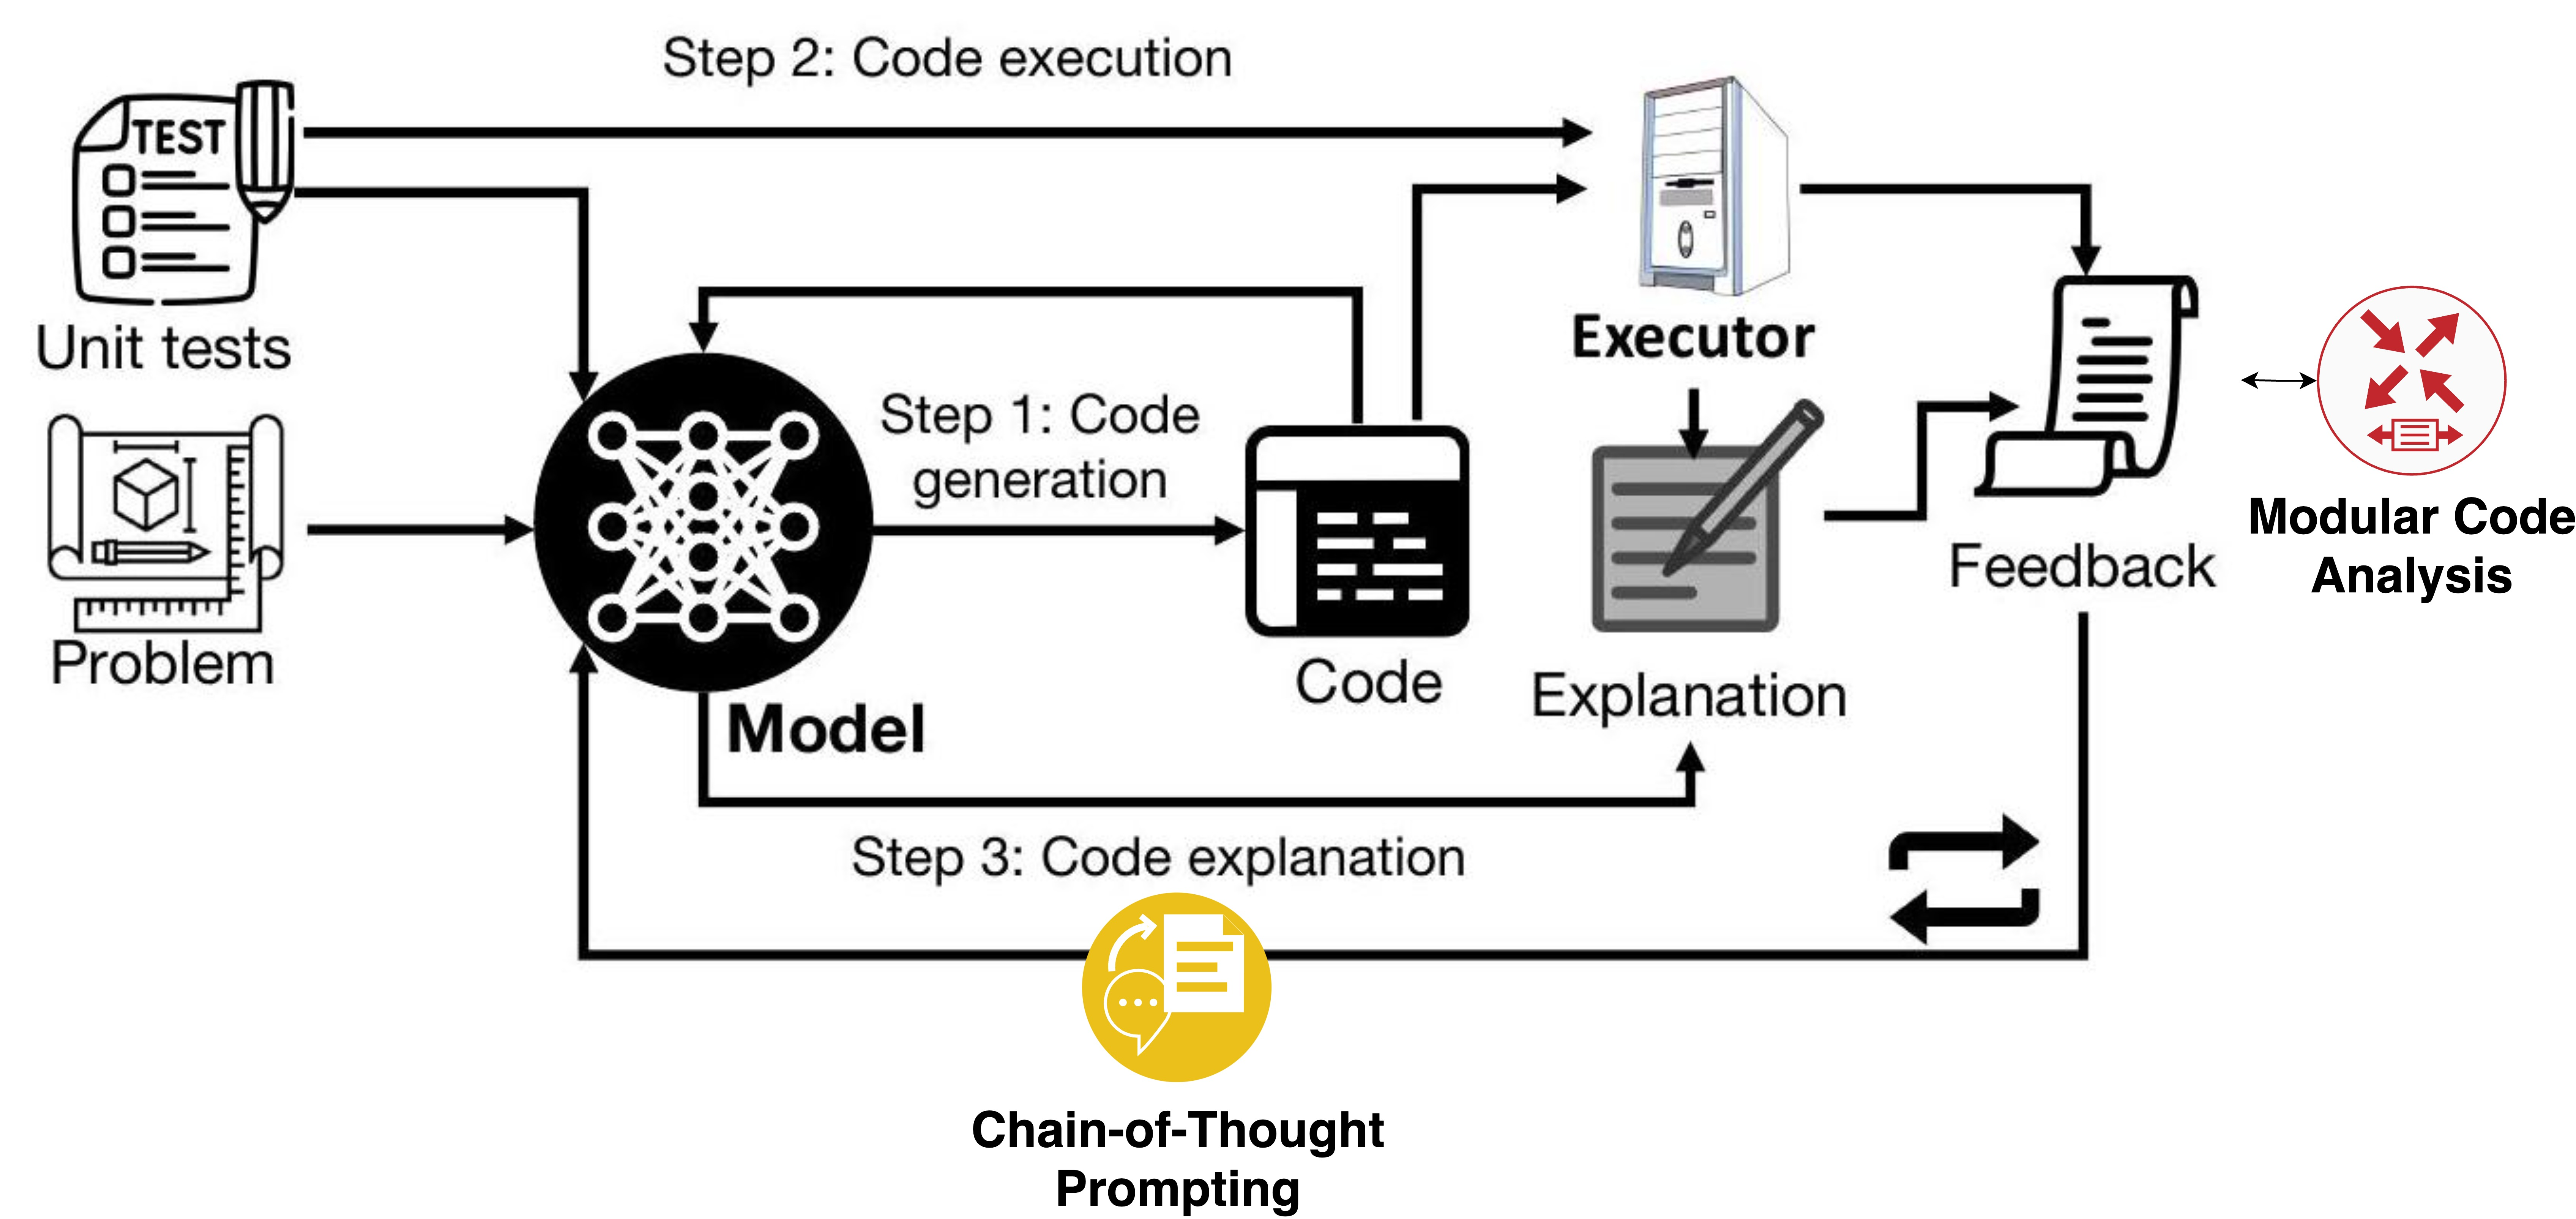
\includegraphics[width=1\textwidth]{img/enhanced_self_debug}
        \captionsetup{font=small,labelformat=empty}
        \caption{Architecture of the proposed system.}
    \end{figure}
\end{frame}

\begin{frame}{Chain-of-Thought Prompting}
    \textit{Chain-of-Thought} (CoT) prompting~\cite{wei2023chainofthought}, which uses a series of intermediate reasoning steps, significantly improves the ability of LLMs to perform complex reasoning.\\
    In this research, CoT prompts are leveraged to explain the debugging process.
    \begin{figure}[!htb]
        \centering
        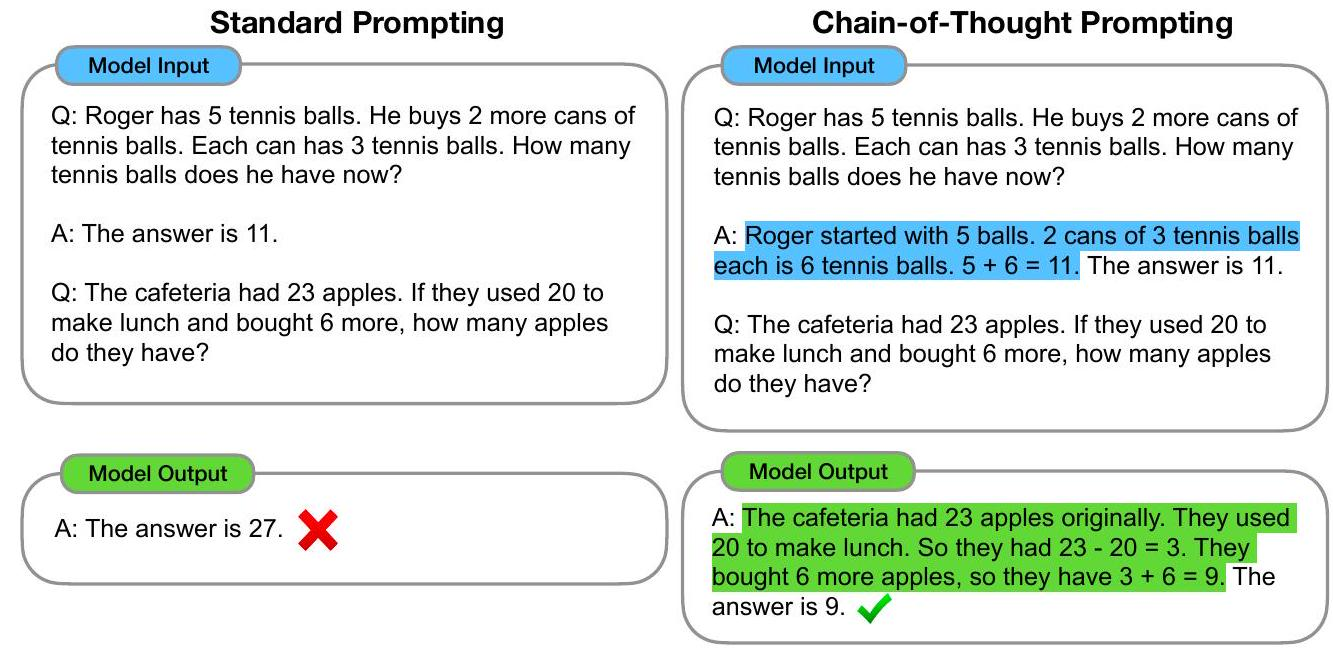
\includegraphics[width=0.75\textwidth]{img/cot_prompting}
        \captionsetup{font=small,labelformat=empty}
        \caption{Chain-of-Thought reasoning processes are highlighted.}
    \end{figure}
\end{frame}

\begin{frame}{Modular Code Analysis}
    Decomposing complex code into manageable subcomponents, an approach known as \textit{Modular Code Analysis} (MCA)~\cite{le2023codechain}, has demonstrated success in code generation tasks.\\
    This research employs MCA to identify related code modules from data science libraries (Pandas, Numpy, etc.) and facilitate comprehension by LLMs.
    \begin{figure}[!htb]
        \centering
        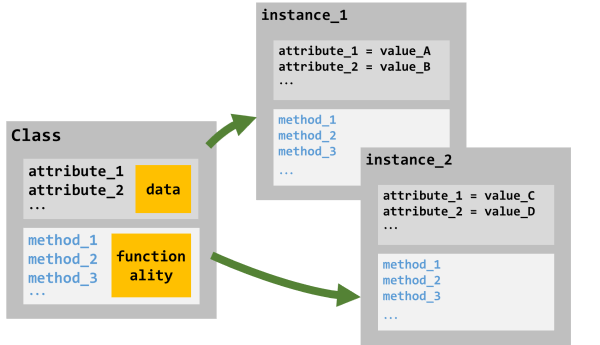
\includegraphics[width=0.55\textwidth]{img/class_diagram}
        \captionsetup{font=small,labelformat=empty}
        \caption{Illustration of code modules.}
    \end{figure}
\end{frame}

\begin{frame}{Dataset}
    DS-1000~\cite{pmlr-v202-lai23b}: 1000 Python data science coding problems, each with:
    \begin{block}{Problem Description}
        \small
        Problem:
        How do I get the dimensions of an array? For instance, this is (2, 2):\\
        a = np.array([[1,2],[3,4]])
    \end{block}

    \begin{columns}[T]
        \begin{column}{0.50\textwidth}
            \begin{block}{Buggy Code}
                \small
                <code>\\
                import numpy as np\\
                a = np.array([[1,2],[3,4]])\\
                </code>\\
                result = $\ldots$ \# put solution in this variable\\
                BEGIN SOLUTION\\
                <code>
            \end{block}
        \end{column}
        \begin{column}{0.45\textwidth}
            \begin{block}{Unit Test}
                \small
                def test(result, ans):\\
                \ \ \ \ assert\_array\_equal(result, ans)\\
                \ \ \ \ return 1
            \end{block}
        \end{column}
    \end{columns}
\end{frame}

\begin{frame}{Evaluation}
    \begin{figure}[!htb]
        \centering
        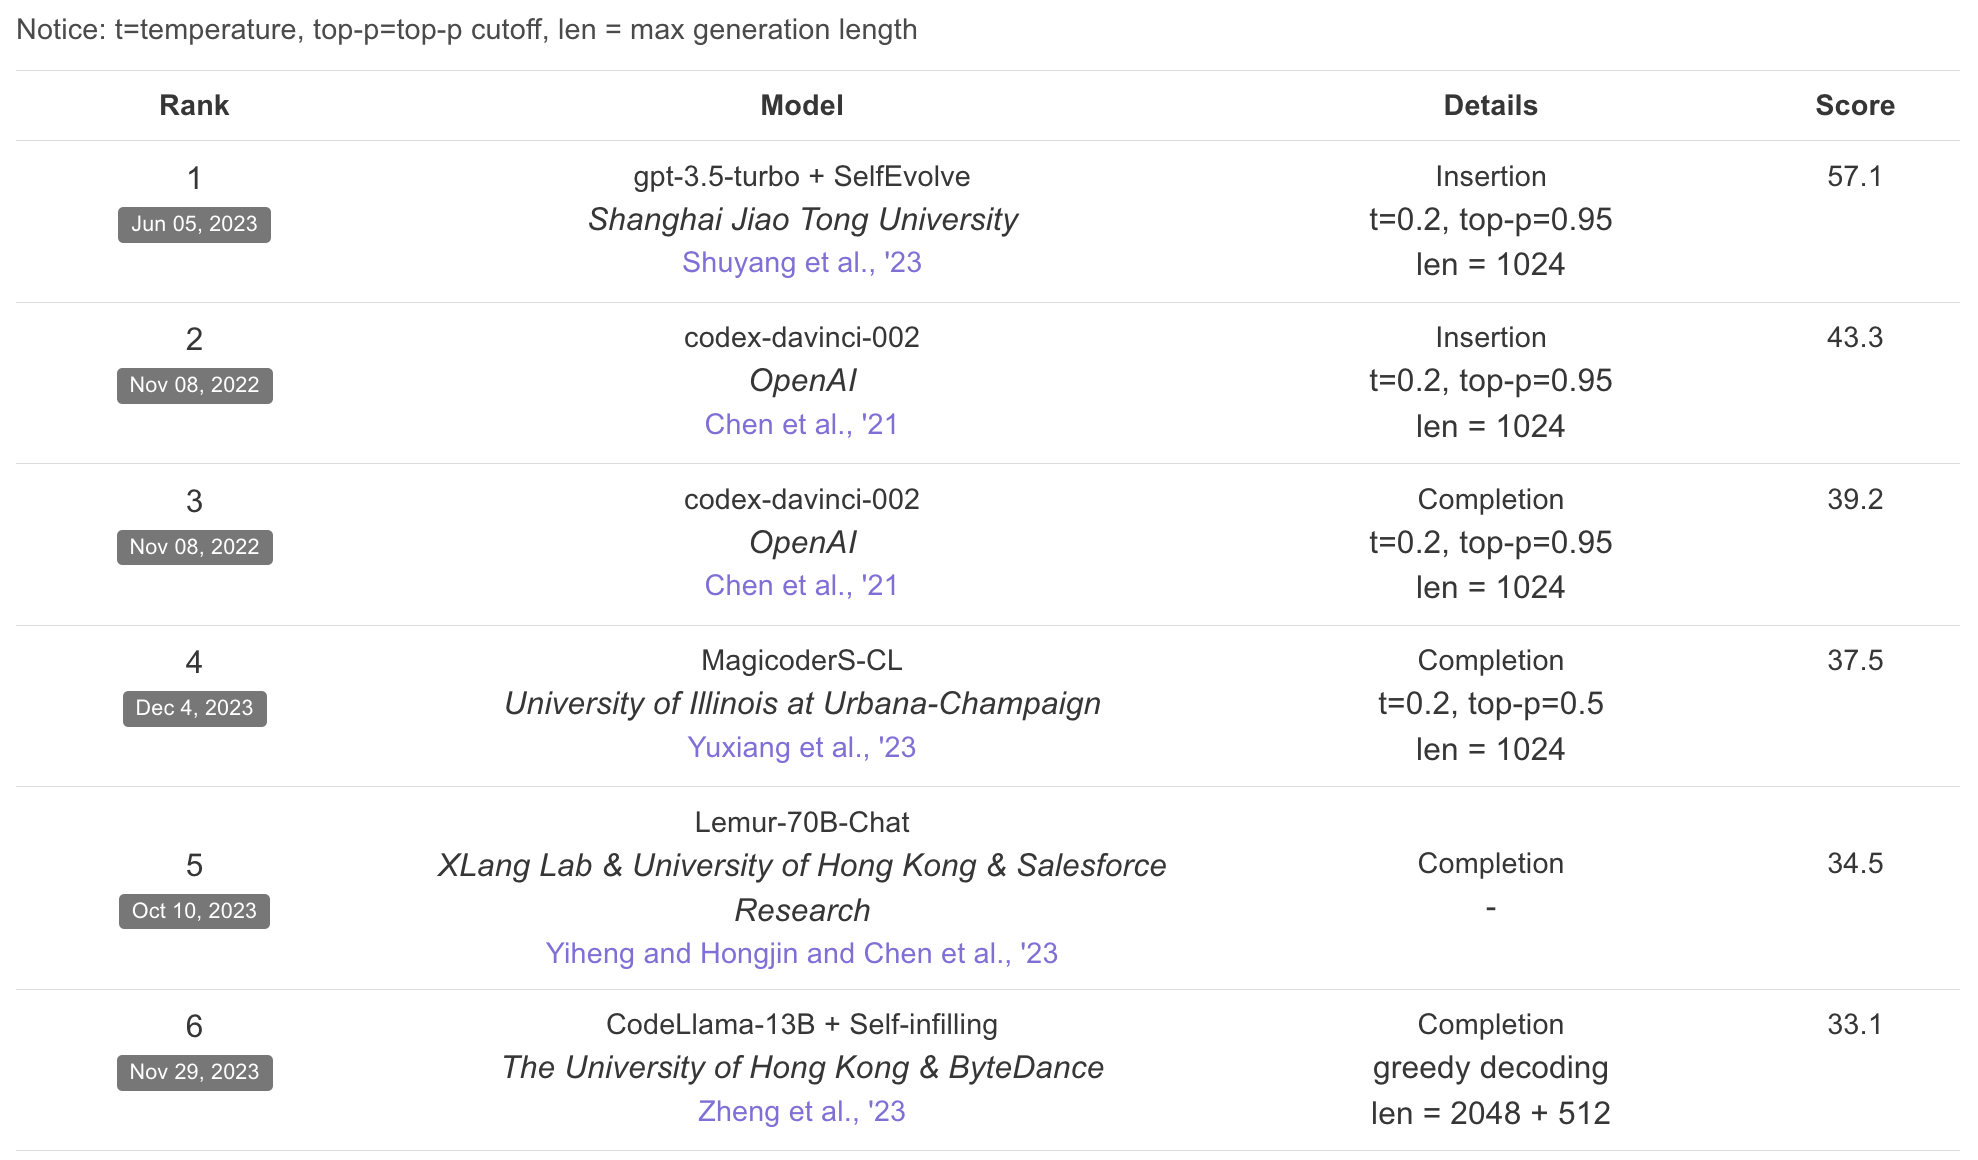
\includegraphics[width=0.9\textwidth]{img/ds1000_evaluation}
        \captionsetup{font=small,labelformat=empty}
        \caption{The current baselines based on DS-1000 dataset.}
    \end{figure}
\end{frame}
